\documentclass{article}
%====================== PACKAGES ======================
\usepackage{wrapfig}
\usepackage{caption}
\usepackage[english]{babel}
\usepackage[utf8]{inputenc}
\usepackage[T1]{fontenc}
\usepackage{titlesec}
\usepackage{pdflscape}
\usepackage{lscape}
\usepackage{rotating}
\usepackage{float}
\usepackage{amsmath}
\usepackage{amsfonts}
\usepackage{amssymb}
\usepackage{graphicx}
\usepackage[colorinlistoftodos]{todonotes}
\usepackage{url}
\usepackage[paper=portrait,pagesize]{typearea}
\usepackage{hyperref}
\hypersetup{
    colorlinks = true,
    linkcolor = black,
    urlcolor = blue }
\usepackage{pdfpages}
\usepackage[final]{pdfpages}
\usepackage{tabularx}
\captionsetup[figure] {
    font = small,
    skip = 5pt }

\usepackage{bm}
\usepackage{algorithm}
\usepackage{soul}
\usepackage{setspace}
\usepackage{abstract}
\usepackage{multicol}
\usepackage{multirow}
\usepackage{paracol}
\usepackage{circuitikz}
\usepackage[nottoc]{tocbibind}
\usepackage{eurosym}
\usepackage{svg}
\usepackage{array}
\usepackage{xcolor}
\usepackage{colortbl}
\usepackage{pifont}
\usepackage{siunitx}
\usepackage{listings}
\usepackage{color}
\usepackage[version=4]{mhchem}
\usepackage{chemist}
\usepackage{fancyhdr}
\usepackage{endnotes}
\usepackage[style=ieee,sorting=none]{biblatex}
\usepackage{csquotes}
\usepackage{comment}
\usepackage{chemfig}
\usepackage{subcaption}
\usepackage[top=1.25cm, bottom=2cm, left=1.75cm, right=1.75cm]{geometry}

%\usepackage{pgfplots}
%\pgfplotsset{compat=2.8}
%\usepgfplotslibrary{statistics}



%====================== DOCUMENT START ======================
\title{
    \begin{figure}[H]
        \centering
        
\includegraphics[width=0.7\linewidth]{politoLogo.png}
    \end{figure}\noindent\\[1cm]
    
    \textbf{Academic Year 2023/2024}\\[1.5cm]
    
    \textsc{Computer Architecture \&\\ Operating Systems}\\[1cm]
    \textbf{HacklOSsim Project}
    \rule{\linewidth}{0.2mm}\\
    \textbf{Project Report}\\[2.25cm]
    

    \huge{Group 20}\\[1cm]
    \large{Sannia Gabriele - S331385\\
    Sabella Mattia Luigi - S285363\\
    Pittalis Domenico - S283602\\
    Nobili Luca - S331461\\}
    
    \date{\vspace{\fill}}
}

\begin{document}
\maketitle
\newpage
\tableofcontents



\newpage
\section{Introduction to FreeRTOS}
\textbf{FreeRTOS} is a \ul{market-leading \textbf{Real-Time Operating System} (\textbf{RTOS}) for microcontrollers} that was released after 18 years of work in partnership with the world’s leading chip companies. Now FreeRTOS is downloaded once every 170 seconds and is distributed freely under the MIT open source license. FreeRTOS includes a kernel and a set of libraries suitable for use across all industry sectors.\\[0.1cm]
FreeRTOS provides robustness, tiny footprint, detailed pre-configured demos, Internet of Things (IoT) reference integrations and scalable size. In addition, FreeRTOS has a minimal ROM, RAM and processing overhead and it is very simple as the core of the RTOS kernel is contained in only three C files.
FreeRTOS provides us with the following \textbf{functionalities}:


\subsection{Tasks}
A real time application that uses a RTOS can be structured as a set of \textbf{independent Tasks}. Since FreeRTOS is designed as a \textbf{single-processor OS}, \textbf{only one} task within the application can be at the Running state at any point in time and the \textbf{Real-Time Scheduler} is responsible for deciding which task this should be. As tasks have \textbf{no knowledge} of the scheduler activity, it is its responsibility to ensure that the \textbf{Context Switch} is performed correctly. To achieve this, each task is provided with its own \textbf{Stack}. Thus, when the task is \textbf{swapped out}, its execution context is saved to the stack of that task so it can also be restored when the same task is later \textbf{swapped in} to continue its execution.\\[0.1cm]
Every time a task is created, a priority level, ranging from \textbf{0} to (\textbf{configMAX\_PRIORITIES - 1}) \textbf{must} be assigned to it. Lower values indicate tasks with lower priority, thus, the \textbf{IDLE Task} has \textbf{always} assigned a priority of \textbf{0} (\textbf{tskIDLE\_PRIORITY}). The scheduler \textbf{must} ensure that tasks in the Ready or Running state always receive CPU time preference over tasks with lower priority that are also in the Ready state. In simpler terms, the task transitioning to the Running state is \textbf{always} the highest-priority task eligible for execution. However, multiple tasks can share the same priority level. Thus, if \textbf{configUSE\_TIME\_SLICING} is either \textbf{undefined} or set to \textbf{1}, Ready state tasks with identical priorities will distribute the available processing time using a \textbf{Time-Sliced Round-Robin Scheduling Algorithm}.


\subsection{Semaphores}
FreeRTOS provides \textbf{Binary Semaphores} and \textbf{Counting Semaphores}. While Binary Semaphores and \textbf{Mutexes} are similar, they differ subtly: Mutexes feature a priority inheritance mechanism, whereas Binary Semaphores do \textbf{not}. Consequently, Binary Semaphores are preferable for \textbf{synchronization tasks}, while Mutexes excel at \textbf{simple mutual exclusion tasks}.\\[0.1cm]
FreeRTOS's Semaphore API functions allow specification of a block time, indicating the maximum duration a task should remain in a Blocked state when attempting to acquire a semaphore. If multiple tasks block on the same semaphore, the highest priority task will be unblocked first when the semaphore becomes available.\\[0.1cm]
Similar to how Binary Semaphores represent Queues of length one, while Counting Semaphores can be visualized as Queues with a length greater than one and are primarily used for:
\begin{itemize}
    \item\textbf{Counting Events}: handlers \textit{'give'} a semaphore for each event occurrence, while tasks \textit{'take'} a semaphore for each event processing;%. The count value represents the difference between the occurred and processed events, with \textbf{0} being desirable at semaphore creation;
    
    \item\textbf{Resource Management}: the count value denotes available resources. Tasks \textbf{must} \textit{'take'} a semaphore by decrementing the count value to obtain control of a resource. When the count reaches \textbf{0}, no free resources are available. Tasks \textit{'give'} back the semaphore upon resource release, incrementing the count value. It is preferable for the count value to be equal to the maximum count value at semaphore creation;
\end{itemize}


\subsection{Queues}
Queues are fundamental for enabling communication between tasks in a multitasking system. They serve as channels through which tasks can exchange messages, facilitating coordination and data sharing. Typically, Queues operate on a first-in-first-out (FIFO) basis, meaning that the data sent earlier is received first. However, it is also possible to send data to the front of the Queue if necessary. Queues can handle both small messages stored directly in C variables and larger messages by passing pointers. This approach also supports variable-sized messages and enables a single queue to receive different message types. Queues can block tasks when they are full or empty, allowing for efficient resource utilization. Overall, FreeRTOS queues provide an intuitive and efficient mechanism for inter-task communication in real-time embedded systems.


\subsection{Event Bits \& Event Groups}
\textbf{Event Bits} (or \textbf{Event Flags}) are used to indicate whether an event has occurred or not. They can be defined as individual bits that take on a specific value to represent the state of an event. For example, an application might define a bit that indicates whether a message has been received and is ready to be processed (1) or if there are no messages waiting to be processed (0).\\[0.1cm]
\textbf{Event Groups} are sets of event bits, where each bit is identified by a bit number. For instance, an event group might include bits representing different states of the application, such as message reception, queuing a message to send to the network, or sending a heartbeat message on the network. The API functions for event groups allow tasks to set, clear, and wait for one or more event bits to be set within an event group. They can also be used to synchronize tasks, creating synchronization points where tasks wait until all other involved tasks have reached their synchronization points.



\section{Examples}


\subsection{Basic Tasks: \textit{"semaphoresAcyclic.c"}}
\begin{minipage}[t]{0.6\textwidth}
    This example uses a Counting Semaphore (sem1) that is created with max value 2 and initial value 0 in order to allow task1 to be executed before task2 and task3, a Binary Semaphore (sem2) and a Mutex (Mutex) to protect the critical section (stdout). The purpose of the exercise is to accomplish the following Acyclic Semaphore Precedence Graph.\\[0.1cm]
    task1, which does \textbf{not} need to synchronize with any other task, releases semaphore sem1 twice after printing, thereby unblocking task2 and task3, both of which subsequently print and release sem2 (Note that just one semaphore to unlock 2 task because the graph is acyclic). Now, task4 (which was supposed to acquire sem2 twice) can print and terminate.
\end{minipage}
\begin{minipage}[t]{0.4\textwidth}\vspace{-50pt}
    \begin{figure}[H]
        \centering
        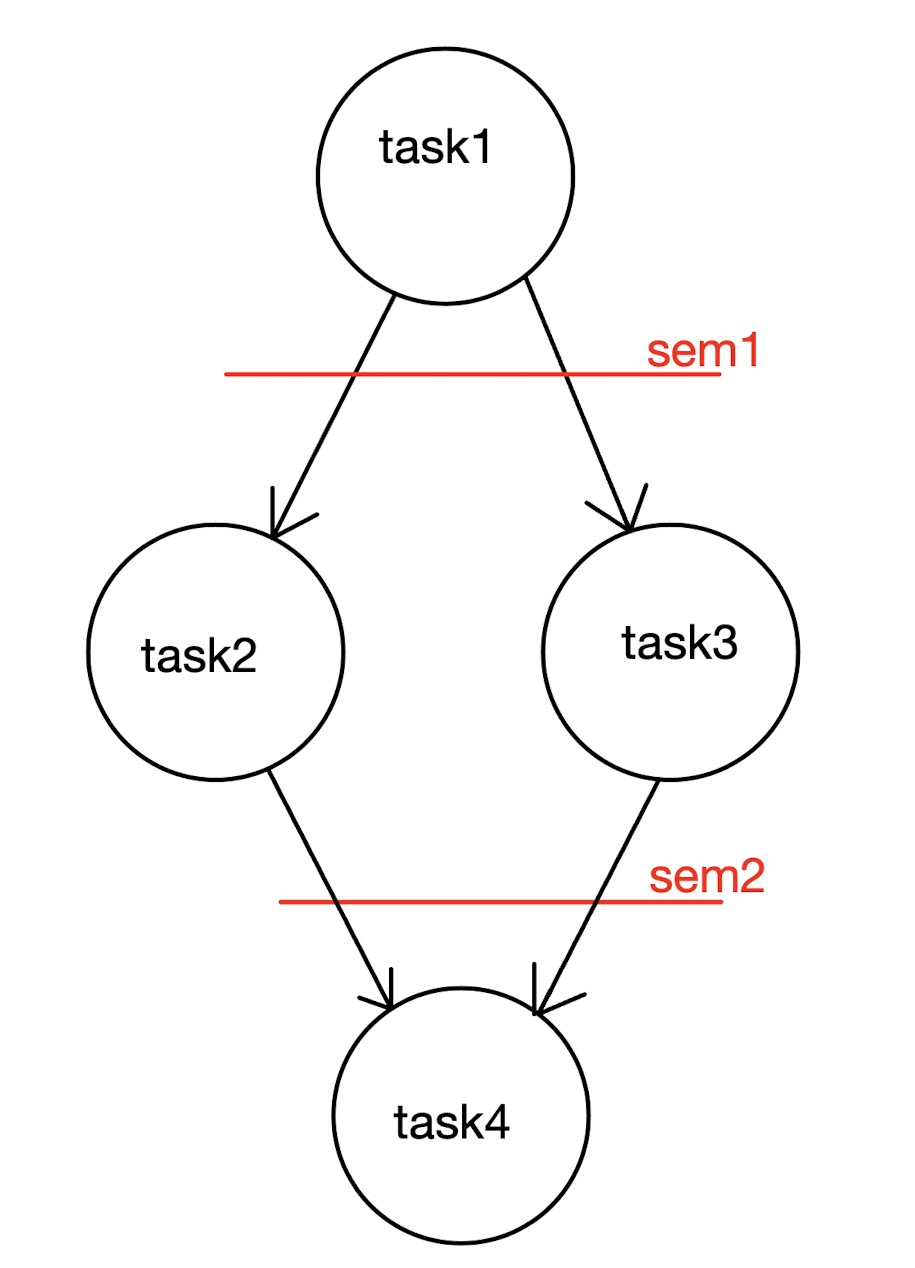
\includegraphics[width=0.65\linewidth]{acyclic.jpeg}
        \caption{Acyclic Semaphore Precedence Graph}
    \end{figure}\noindent
\end{minipage}


\subsection{Extended Tasks: \textit{"semaphoresCyclic.c"}}
\begin{minipage}[t]{0.6\textwidth}
    The substantial difference from the previous example is that here \textbf{Extended Tasks} are implemented, leading to the creation of a Cyclic Semaphore Precedence Graph. However, it is not possible for one task to unblock two other tasks using the same semaphore, for this reason task2 and task3 require two independent semaphores (if they were to share the same semaphore, it could happen that one of the tasks acquires it twice while the other does not acquire it at all).\\[0.1cm]
    Another peculiarity to note is that task1 (being the first to execute) is the only task whose semaphore (another even more than the previous example) has a value of 1 upon its creation; otherwise, the tasks would all remain permanently blocked.\\[0.1cm]
    
\end{minipage}
\begin{minipage}[t]{0.4\textwidth}\vspace{-65pt}
    \begin{figure}[H]
        \centering
        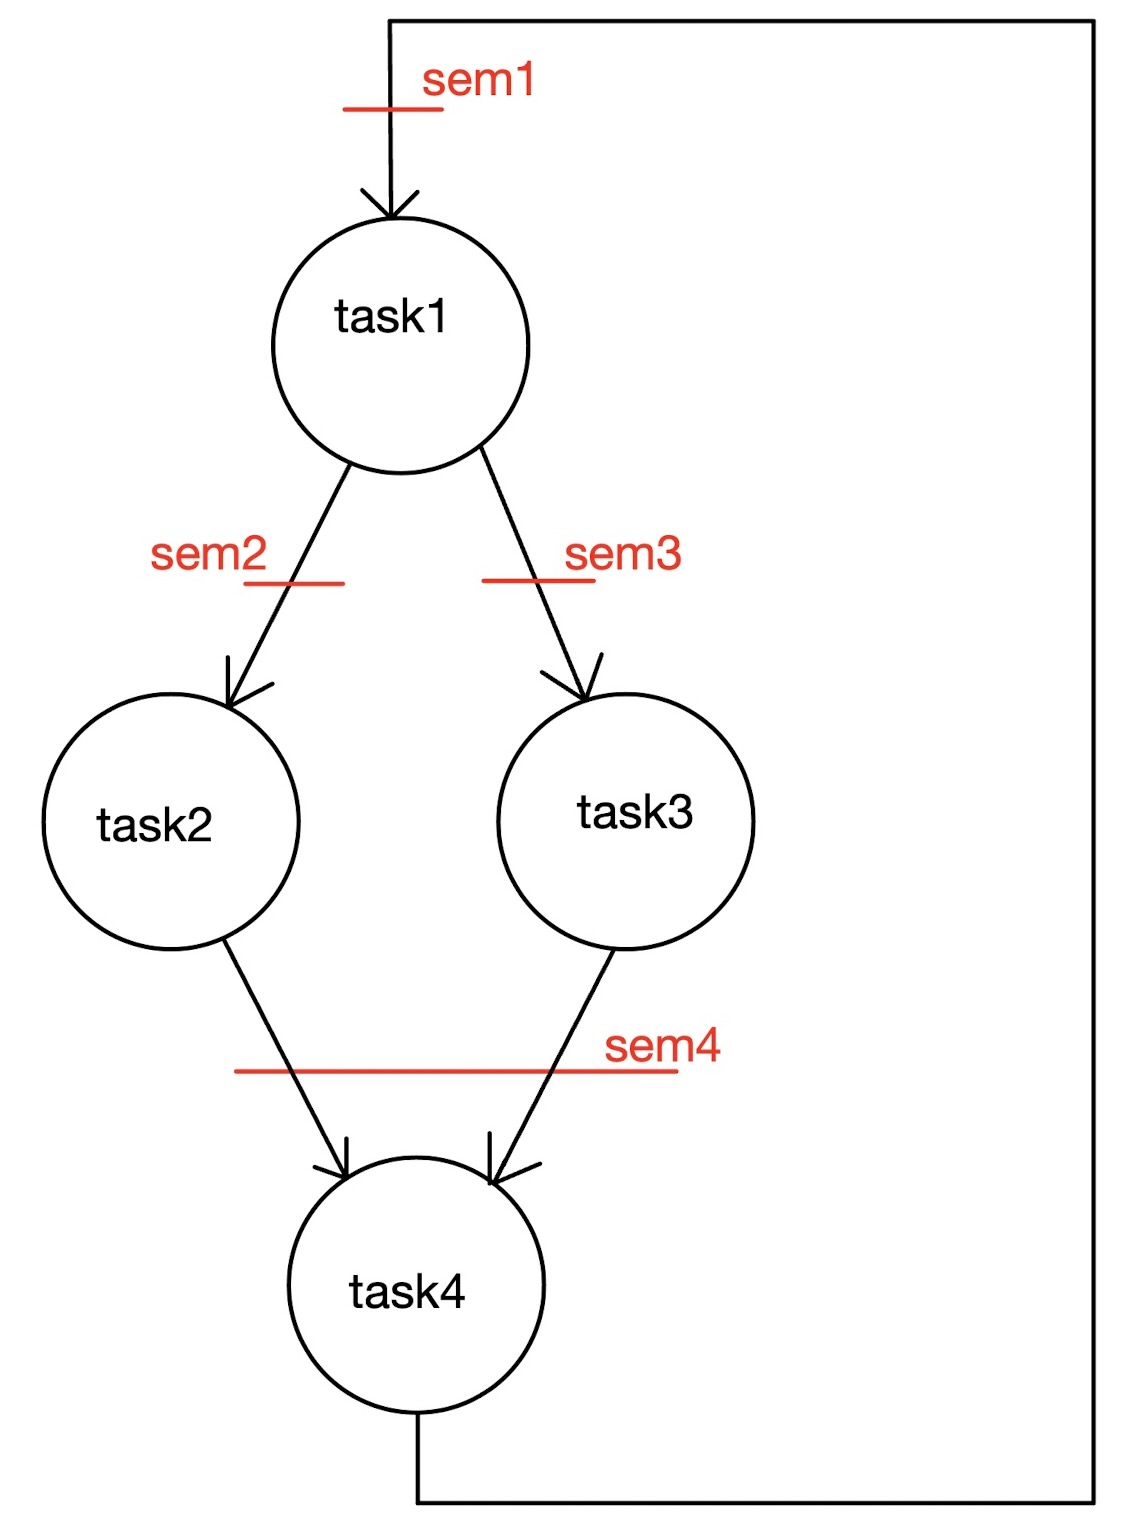
\includegraphics[width=0.8\linewidth]{cyclic.jpeg}
        \caption{Cyclic Semaphore Precedence Graph}
    \end{figure}\noindent
\end{minipage}


\subsection{Queue: "\textit{queueChar.c}"}
In the \textit{\textbf{"queueChar.c"}} example script, our aim is to demonstrate how FreeRTOS handles two tasks that try to work \textbf{concurrently} using Queues. The code creates two tasks: \textbf{queueSendTask} and \textbf{queueReceiveTask}, both with the same priority, which send and receive characters via a queue, for this reason the Round-Robin is used.\\[0.1cm]
The \textbf{queueSendTask} task sends characters from a string defined as global to the queue one by one at regular intervals of 200 milliseconds.\\[0.1cm]
The \textbf{queueReceiveTask} task receives characters from the Queue and prints them to the console, with a delay of 500 milliseconds between each received character.
\begin{figure}[H]
    \centering
    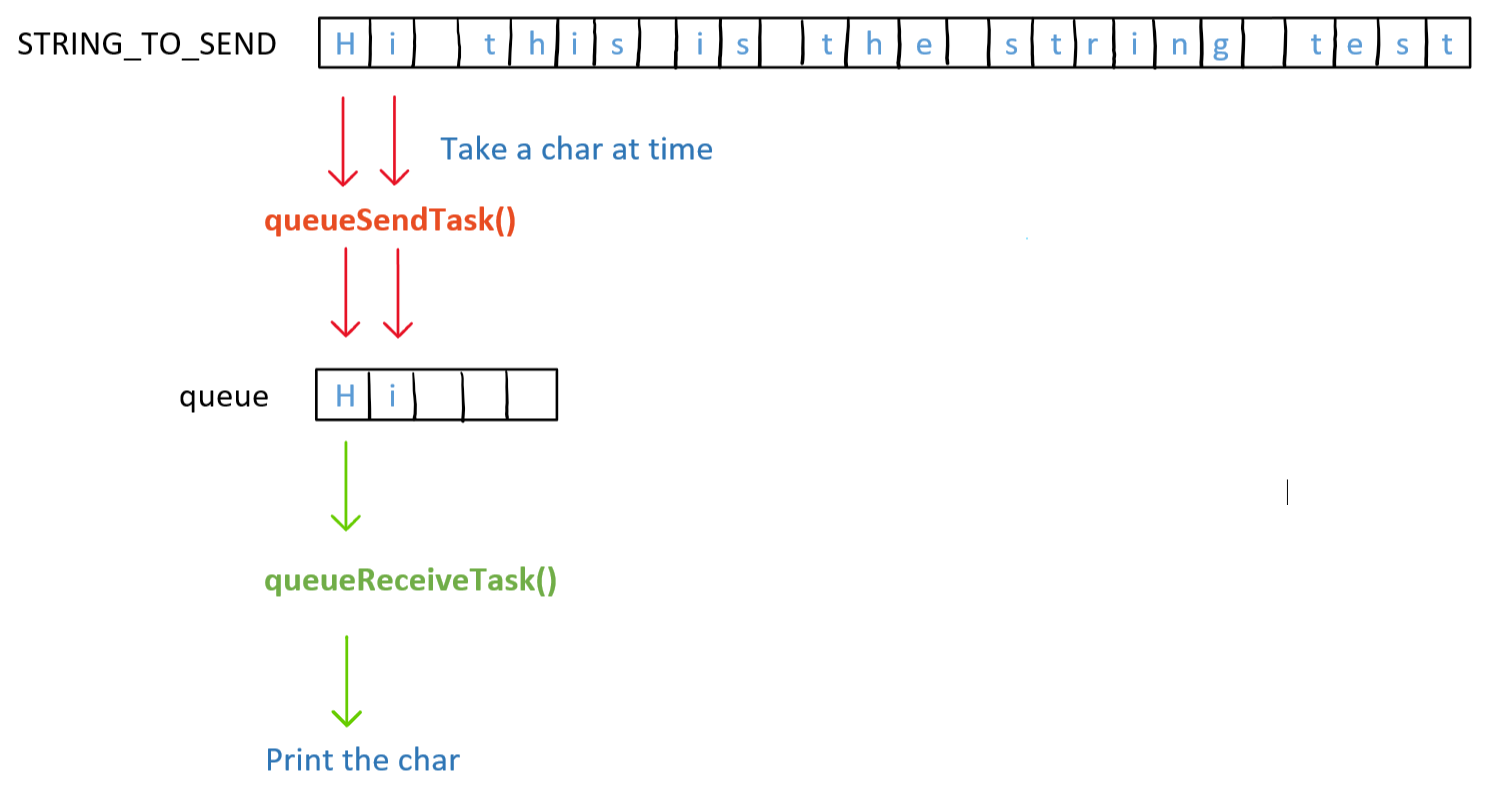
\includegraphics[width=0.8\linewidth]{queue.png}
    \caption{Queue Example}
\end{figure}\noindent


\subsection{Event Group: "\textit{event2Tasks.c}"}
The example \textit{\textbf{"event2Tasks.c"}} shows how to coordinate the concurrent execution of different tasks using \textbf{eventGroup}s. The code defines three main tasks: \textbf{Task1}, \textbf{Task2}, and \textbf{Task3}.\\[0.1cm]
\textbf{Task1} takes care of the initialization of the system. Essentially, it creates an event group (\textbf{eventGroup}) that is used to coordinate the execution of tasks. \textbf{Task1} then creates \textbf{Task2} and \textbf{Task3} that alternate their execution. Initially, \textbf{Task1} notifies \textbf{Task2} to start it. Once this is done, \textbf{Task1} finishes executing.\\[0.1cm]
\textbf{Task2} and \textbf{Task3} form the core of multitasking. They wait for the turn event respectively and when it is received, they perform their specific task (printing a message in the specific case). After completing their task, each task notifies the next task in the loop of the event so that it can execute.
\begin{figure}[H]
    \centering
    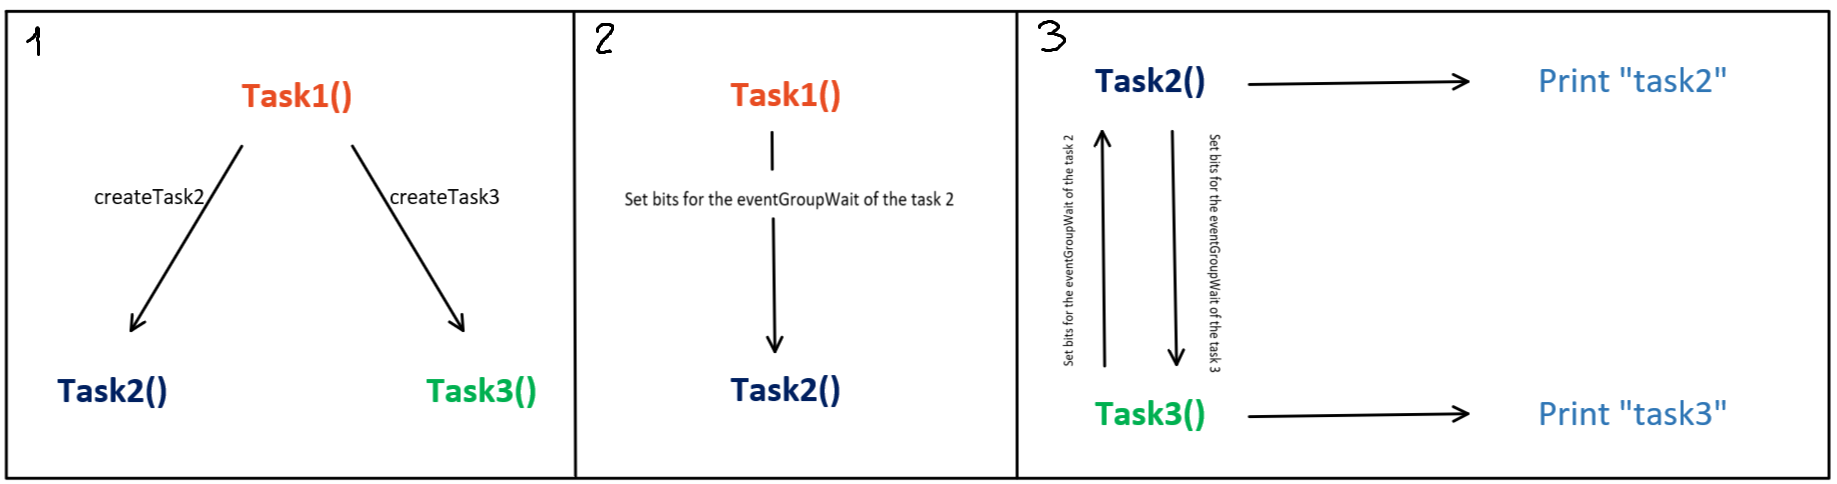
\includegraphics[width=\linewidth]{EventGroup.png}
    \caption{EventGroup Example}
\end{figure}\noindent



\section{EDF Scheduler}
The \textbf{Earliest Deadline First} (\textbf{EDF}) algorithm is a \textbf{scheduling policy} used in real-time systems to schedule tasks based on their deadlines. EDF assigns priorities to tasks \textbf{dynamically}, with the task having the earliest deadline being given the highest priority. This ensures that tasks with closer deadlines are executed first, reducing the likelihood of missing deadlines. Additionally, EDF uses \textbf{preemption} which ensures that higher-priority tasks can interrupt the execution of lower-priority tasks when necessary\\[0.1cm]
In implementing the EDF algorithm, our \textbf{primary objectives} were to maintain FreeRTOS's original structure as possible and handle aperiodic tasks as \textbf{soft real-time systems} with a \textbf{Background Scheduling} approach. This entails scheduling aperiodic tasks based on their arrival order, ensuring execution when no other periodic tasks are in the ready list. Furthermore, ensuring system feasibility is crucial to enable the scheduling algorithm to operate effectively.\\[0.1cm]
All the changes we are about to illustrate pertain to the \textit{\textbf{"tasks.c"}} file. To allow a user to select among the various scheduling algorithms of FreeRTOS, including the one we propose, we added \textbf{configUSE\_EDF} to \textit{\textbf{"FreeRTOSConfig.h"}}. By setting it to \textbf{1}, the EDF scheduler will be used.\\[0.1cm]
As mentioned earlier, our scheduling requires knowledge of the \textbf{deadlines} for each task in order to schedule them correctly. For this reason, a proper parameter has been added to the Task Control Block (TCB). Therefore, a new task creation function that allows passing the deadline as a parameter is necessary.\\[0.1cm]
The new function is called \textbf{xTaskCreateEDF} and, as previously mentioned, it accepts a parameter of type \textbf{TickType\_t} for the deadline. Additionally, within it, the value is saved through a pointer to the TCB, which will be used later to calculate the priority associated with the task. Our EDF  structure entails that the priority (hence the deadline) of a task resides in the \textit{Item} linked to the \textbf{xStateListItem}. Thus, using a pre-implemented function, \textbf{listSET\_LIST\_ITEM\_VALUE}, we set the current tick as the initial value, which before calling \textbf{vTaskStartScheduler} will be \textbf{0}.
\noindent% C'è bisogno di ripetere che "xStateListItem" fa parte del TCB?
The \textbf{xStateListItem} is a data structure used internally by FreeRTOS to manage task state information. It is a member of the TCB. By utilizing \textbf{xStateListItem}, containing information about the task's state and its reference to the state list, we can dynamically track the task's priority.\\[0.1cm]
FreeRTOS normally uses multiple lists to manage tasks. However, for our scheduler, we prefer \textbf{simplicity}. So, we've decided to use just one list. This list will arrange tasks based on their deadlines (the \textbf{listItem} in \textbf{xStateListItem} mentioned before), with the closest deadline at the top. To make this happen, we've created a new list called \textbf{xReadyTasksListsEDF}.\\[0.1cm]% di quale file si sta parlando?
With the changes made so far, we've successfully created a task that accepts the deadline as a parameter, saves it in the TCB, and sets it as the initial parameter of the \textbf{xStateListItem}. Additionally, we've created the new ready list.\\[0.1cm]
The next modification deals with how deadlines and priorities are updated. To achieve this, we've modified the \textbf{prvAddTaskToReadyList} function, responsible for inserting tasks into the ready list, in order to update the deadline every time a task needed to be inserted into the ready list. Firstly, we calculate the new deadline by adding the value of the previous deadline contained in the \textbf{xStateListItem}'s item to the declared deadline in the task creation, which had been saved in the TCB.\noindent
Subsequently, we set the new value of the \textbf{xStateListItem}'s item using \textbf{listSET\_LIST\_ITEM\_VALUE}. Finally, we call the \textbf{vListInsert} function (originally from FreeRTOS), which positions our task within the ready list according to the ascending order of deadlines.\\[0.1cm]
The management of \textbf{IDLE tasks} is also revised. Initialization of the IDLE task occurs within the \textbf{vTaskStartScheduler} method.\\[0.1cm]
In the standard FreeRTOS scheduler, the IDLE task is a straightforward task initialized with the lowest priority. Consequently, it is scheduled \textbf{only} when no other tasks are ready. However, with the EDF scheduler, the lowest priority behavior can be simulated by assigning a task with the farthest deadline. Therefore, a high value (e.g. \textbf{1000000}) is assigned as the deadline.\\[0.1cm]
 The next required adjustment involves the \textbf{context switching mechanism}. In the function \textbf{vTaskSwitchContext} with the FreeRTOS scheduler, a dedicated function was used to retrieve the highest priority task. With the new ready list, it will be sufficient to fetch the task at the head of it using the function \textbf{listGET\_OWNER\_OF\_HE}-\\\textbf{AD\_ENTRY} which is already implemented in FreeRTOS, as it is used by other functions that work on lists like ours for EDF (e.g. delayed List). Given the memory address of the ready list, this function returns the TCB of the new task to be executed.\\[0.1cm]
 To enable preemption, an additional step is necessary. We need to specify when the context switching is required after a task returns to the ready list (for example, when it exits from the delayed list associated with \textbf{vTaskDelay}). Therefore, in the \textbf{xTaskIncrementTick} task, for each tick, it is checked whether a task returns to the ready list or not. Consequently, the deadlines of the new task inserted into the ready list are compared with those of the task in execution (the deadlines are contained in the \textbf{xStateListItem} explained earlier). If the deadline of the task just reinserted into the ready list is strictly less than that of the task in the running state, the variable \textbf{xSwitchRequired} is set to \textbf{True}, indicating that a context switch is necessary. The decision to use \textit{'strictly less than'} rather than \textit{'less than or equal to'} is based on the fact that it reduces the number of context switches performed. It is easy to see that if two tasks have the \textbf{same deadline}, it is inefficient to execute a swap of the running state.\\[0.1cm]
To manage the aperiodic tasks, it was decided \textbf{not} to use a new ready list. Instead, to allow for a \textbf{simpler} and \textbf{more intuitive} structure, the same ready list as the periodic tasks is utilized. In fact, a \textbf{Background Scheduling} based on the arrival order is created by placing these tasks slightly below the fictitious deadline of the IDLE task. This ensures that they are executed when there are no other periodic tasks. Therefore, a dedicated \textbf{vTaskCreate} function has been created for them, where their "deadline" is set following a counter that defines their arrival order (\textbf{taskIDLEdeadline - count}). This means that the number of aperiodic tasks is limited to the value of the counter. For this reason, it was chosen to allow the user to set this parameter in the \textit{\textbf{"FreeRTOSConfig.h"}} file.


\subsection{Performance Evaluation \& Comparison}
To demonstrate the functionality of the EDF scheduler with aperiodic tasks, the \textit{\textbf{"main\_edf.c"}} demo was created containing two periodic tasks and two aperiodic tasks, \ul{assuming coinciding periods and deadlines}. The two periodic tasks, \textbf{TaskA} and \textbf{TaskB}, have periods of 40 and 70 ticks respectively, with Worst-Case Execution Times (WCET) of 20 and 30. The aperiodic tasks, \textbf{TaskC} and \textbf{TaskD}, have a WCET of 10. To demonstrate their correctness, the software Cheddar was used. Cheddar is a GNU GPL real-time scheduling simulator and schedulability tool. The \textit{\textbf{"main\_edf\_aperiodic.c"}} demo with \textbf{only} periodic tasks is also provided.
\begin{figure}[H]
    \centering
    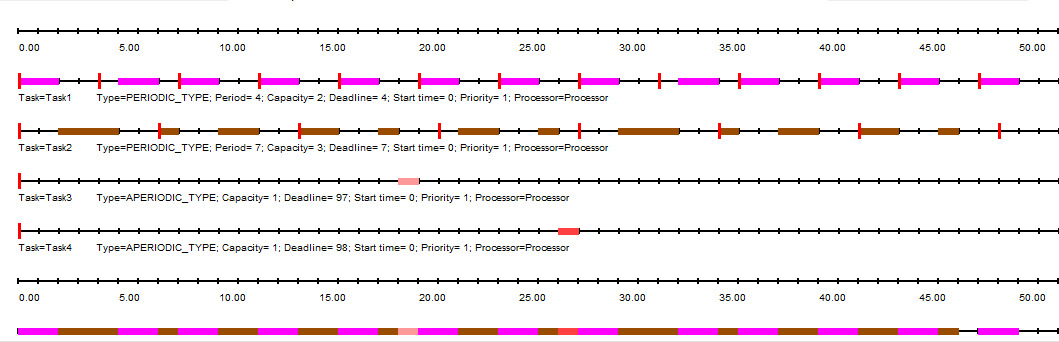
\includegraphics[width=\linewidth]{cheddar_edf_aperiodic.png}
    \caption{EDF Scheduler Performance Evaluation}
\end{figure}\noindent



\section{Multilevel Queue Scheduler}
The implemented \textbf{Multilevel Queue Scheduler} utilizes the five Ready Lists of the basic FreeRTOS scheduler, where each list is associated with a different priority: the first four lists, including the one containing the IDLE task, operate based their priorities with preemptive scheduling and \textbf{without} time slicing. While the fifth list, which has the highest priority, works using Round-Robin.\\[0.1cm]
Thus, a Context Switch can happen \textbf{only if one or more} of the following conditions are true:
\begin{itemize}
    \item A higher priority task enters the Ready Lists;
    \item The Running Task is suspended (which means it is removed from the its Ready List);
    \item The time-slice of the task is finished;
\end{itemize}
When a task is suspended and exits its Ready List, its initial priority is restored. To achieve this, the \textbf{UBaseType\_t uxOldPriority} variable is added to the TCB to store the old priority of the task. On top of that, the \textbf{int cc} variable is also added to the TCB, but it has \textbf{only} an internal purpose.\\[0.1cm]
The \textbf{xTaskIncrementTick} function has been modified in order to:
\begin{itemize}
    \item Implement round-robin on the highest priority list, which is activated \textbf{only} when there are \textbf{at least} two task inside it;

    \item Restore the priority of a task when it is reinserted into the appropriate Ready List;

    \item Mitigate \textbf{Starvation} of low priority task through the implementation of an \textbf{Aging} mechanism: every \textbf{tick\_update\_rate} ticks, all tasks (except the running one) in the first four Ready Lists will get their priority increased by \textbf{1}, until they reach the highest priority list.\\[0.1cm]
    This increment is operated, each time the system tick counter reaches a multiple of the \textbf{tick\_update\_rate}, by the \textbf{xTaskPrioritySet} function (a modified version of the \textbf{vTaskPrioritySet} function);
\end{itemize}  


\subsection{Performance Evaluation \& Comparison}
In the \textit{\textbf{"main\_prova\_mlq.c"}} demo, two tasks are used: \textbf{Task1} with priority \textbf{3}, which is \textbf{never} suspended, and \textbf{Task2} with priority \textbf{1}. At the end of its execution, \textbf{Task2} is suspended for 10 ticks and then placed back in the Ready List, for three times. This demo allows us to show:
\begin{itemize}
    \item How priority is increased every time that the system tick is a multiple of the \textbf{tick\_update\_rate};

    \item The restoration of the old priority of \textbf{Task2} once it is re-inserted in the Ready List;

    \item The activation of round-robin when both tasks are in the highest priority list;
\end{itemize}



\newpage
\section{Work Contributions}
\begin{enumerate}
    \item Gain proficiency in using QEMU for running an embedded operating system and create a tutorial detailing the installation and usage procedures: 
    \begin{itemize}
        \item General understanding of the installation and usage procedures of QEMU and FreeRTOS:
        \begin{itemize}
            \item Sannia Gabriele - S331385
            \item Sabella Mattia Luigi - S285363
            \item Pittalis Domenico - S283602
            \item Nobili Luca - S331461
        \end{itemize}

        \item Creation of the \textit{\textbf{Step-by-Step Installation Guide.pdf}}:
        \begin{itemize}
            \item Sannia Gabriele - S331385
            \item Pittalis Domenico - S283602
        \end{itemize}
    \end{itemize}

    \item Develop practical examples/exercises demonstrating the functionality of the simulator/operating system in alignment with the topics studied in class:
    \begin{itemize}
        \item General understanding of the main FreeRTOS functionalities (e.g. task creation and management):
        \begin{itemize}
            \item Sannia Gabriele - S331385
            \item Sabella Mattia Luigi - S285363
            \item Pittalis Domenico - S283602
            \item Nobili Luca - S331461
        \end{itemize}

        \item Creation of the \textit{\textbf{Project Presentation group20.pptx}} and \textit{\textbf{HacklOSsim Report.pdf}} relating the main FreeRTOS functionalities:
        \begin{itemize}
            \item Sannia Gabriele - S331385
            \item Sabella Mattia Luigi - S285363
        \end{itemize}
    \end{itemize}

    \item Customize the operating system to implement a new solution (e.g., scheduling, memory management, etc.):
    \begin{itemize}
        \item EDF Scheduler implementation:
        \begin{itemize}
            \item Sabella Mattia Luigi - S285363
            \item Nobili Luca - S331461
        \end{itemize}

        \item Multilevel Queue Scheduler implementation:
        \begin{itemize}
            \item Sannia Gabriele - S331385
            \item Nobili Luca - S331461
        \end{itemize}
    \end{itemize}

    \item Evaluate and benchmark the performance improvement achieved by the newly implemented solution:
    \begin{itemize}
        \item EDF Scheduler Demo creation:
        \begin{itemize}
            \item Sannia Gabriele - S331385
            \item Pittalis Domenico - S283602
            \item Nobili Luca - S331461
        \end{itemize}

        \item Multilevel Queue Scheduler Demo creation:
        \begin{itemize}
            \item Nobili Luca - S331461
        \end{itemize}
    \end{itemize}
\end{enumerate}



\end{document}
%====================== DOCUMENT END ======================